% Chapter X

\chapter{Anomaly Detection in Distributed Tracing Data} % Chapter title

\label{ch:traces} % For referencing the chapter elsewhere, use \autoref{ch:name} 
\minitoc
\bigskip

In ~\autoref{ch:logs} we presented analysis of log data in detail. Significant failures in complex distributed systems infrequently occur because of one particular event happening in one specific component of the system. As logs and metrics are system scoped, it is difficult to correlate events across system components. This represents the strongest drawback of log and metric data. Systems based on distributed architectures consists of several services connected by a network. To monitor the user requests with a detailed description of different participating microservices, distributed tracing technologies are utilized. Tracing technologies~\cite{36356, kaldor2017canopy,Fonseca:2007:XPN:1973430.1973450} generate spans to externalize the state of the system by combining performance data from the end-to-end execution path with structured and causally related execution traces. In other words, the tracing data consists of two modalities (1) service response time in the form of real-valued data, and (2) causal relationships with other related services represented as a sequence of textual labels. As shown in Figure \ref{fig:traces}, if user request (e.g., create virtual machine) involves the services $\{11, 21, 31, 32\}$, then a trace contains events representing the intra-service calls produced when each service is invoked. 

\begin{figure}[!t]
\centerline{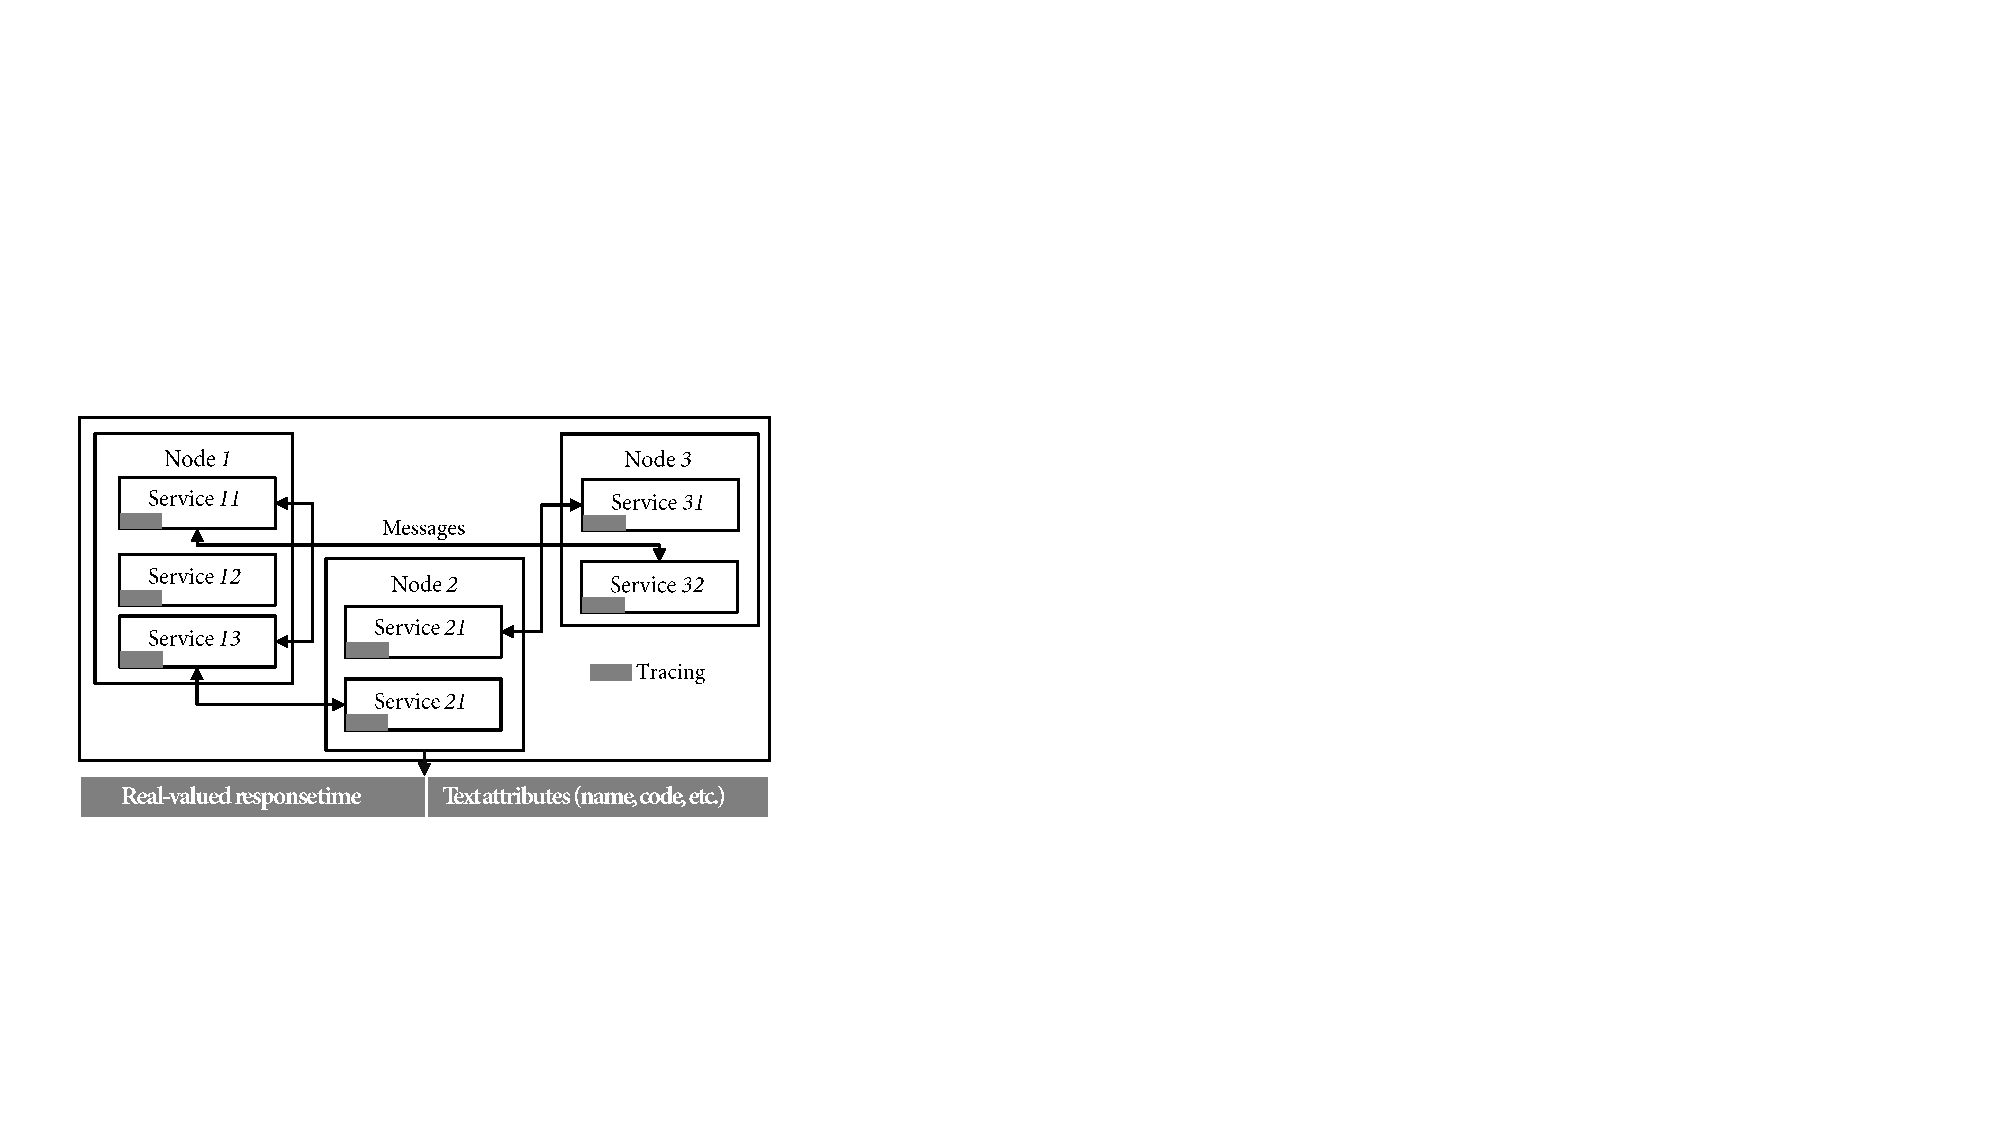
\includegraphics[scale=1.0]{gfx/chap6/tracingshowcase.pdf}}
\caption{Overall system architecture showing communication between services and the tracing system observability component.}
\label{fig:traces}
\end{figure}

The tracing data and its complexity, as described in~\autoref{ch:concepts:sec:anomalydetectionindistributedsoftwaresystems:subsec:trace}, pose challenges to the traditional methods~\cite{chow2014mystery}.
The performances of traditional algorithms in detecting anomalies is known to be low on sequence datasets with high dimensional representations, as they cannot capture complex patterns~\cite{pang2020deep}. As the volume of data increases, for example, to gigabytes per second, it becomes hard for the traditional methods to scale to such large-scale data to find anomalies~\cite{chalapathy2019deep}.

Therefore, we transfer and compile the tracing data into an abstract structure, which is similar to structures for anomaly detection in processes, logs, natural languages, or any sequential data in order to exploit and improve sophisticated analysis methods developed in these domains. 

In this chapter, we view the trace as a text sentence, where each word corresponds to a span. We learn a "language" model of the traces which later is used for anomaly detection.

During the work carried out in this thesis and published in~\cite{nedelkoski2019anomaly,nedelkoski2019anomalymultimodal}, we present an approach for trace anomaly detection based on LSTM networks~\cite{hochreiter1997long}. By learning to predict next/missing spans in the trace we model the normal behavior of the system. During test time, the idea is if we are unable to successfully predict the next/missing spans, the trace represents anomalous behavior, otherwise it is normal.

%how multimodal trace data can improve the anomaly detection
The current state-of-the-art systems for anomaly detection from system data, model the normal system behavior out of a single data type, which is either the textual log keys, or real-valued performance parameters. Commonly, they use separate models for both types of data and build an ensemble to generate the final prediction~\cite{du2017deeplog}. Other approaches operate solely on one data modality~\cite{8456348, 8457902} or apply separate modeling techniques for multiple modalities, which are later integrated into an unified indicator~\cite{fu2009execution}. However, such additive models do not utilize the existing correlation between the data sources. They learn the normal system behavior from partial and limited data which might affect the overall performance. The learning from fused representations of multimodal data has provided good results in various tasks, matching or outperforming other deep learning models \cite{srivastava2012multimodal}.

To exploit both, the response time and the structural information, we present a novel method, denoted as MiTrace. It learns a model of normality from the joint information in the data and uses it to detect deviations. Furthermore, checking for existing dependencies between the services (such as sequential or parallel execution) is useful for later tasks such as root-cause analysis. MiTrace, enables reconstruction of the learned execution path. This allows for dependency checks and detection of concurrent or sequential events.


Parts of this chapter are published in ~\cite{nedelkoski2019anomalymultimodal,nedelkoski2020data,nedelkoski2019anomaly,nedelkoski2020selftracing}. We summarize the contributions in this chapter in the following, together forming part of a trace anomaly detection system. 
\begin{itemize}
    \item We introduce the task of deep anomaly detection for the domain of distributed traces.
    \item We present a method to detect execution path anomalies that take into account all services involved into serving a particular user request.
    \item We discuss the importance of the response time and propose its inclusion into a joint multimodal method for anomaly detection, called MiTrace. The method learns existing correlations between the execution path and the sequence of response times of the services. 
    \item Lastly, an approach for checking dependencies between events is presented.
\end{itemize}


\section{MiTrace: Multimodal Anomaly Detection from Traces}\label{methodology}
This section explains the parsing of the tracing data, single-modality LSTM network for structural anomaly detection, its extension to the multimodal LSTM neural network, and describes the method for detection of concurrent or dependent events. Both proposed approaches for anomaly detection model the normal system behavior and detect anomalies by flagging deviations.

\textbf{Formal definition.} Consider a set of historical traces $\mathcal{X_t} = \mathbf{x_{1}}, \mathbf{x_{2}}, \dots, \mathbf{x_{N}}$, where $N$ is the size the set and $\mathbf{x_{1}}, \mathbf{x_{2}}, \dots, \mathbf{x_{N}}$ are observed traces. Each trace $\mathbf{x_{i}}$ is composed of events/spans that contain textual and response time information $\mathbf{x_{i}}= (x_{text}, x_{rt})$. Let $\phi(\mathbf{x_i}, \theta)$ be a function represented by a neural network, which first maps the input to a latent representation in $\mathbb{R}^h$, and then to a right-shifted input, representing the output of the network $\mathbf{x_{i}-shifted}$. The task is to learn the parameters $\theta$, and then for each incoming instance in the prediction phase $\mathbf{x_1^{test}}, \mathbf{x_2^{test}},\dots, \mathbf{x_i^{test}}, \dots\}$, predict whether it is anomaly or normal based on the reconstruction error scores and a threshold $\tau$.

\subsection{Trace preprocessing}\label{datarepresentation}

A trace $\mathbf{x_{1}}=\{(x_{text}, x_{rt})_1, (x_{text}, x_{rt})_2, \dots, (x_{text}, x_{rt})_m\}$, where $m$ is the length of the trace (number of events), is represented as an enumerated collection of events sorted by the timestamps. The analogy to the natural languages as type of sequential data originates from this representation, where one can map the trace to a sequence of words, the events inside a trace to words, and the causal relationship between events to a language grammar. Each event in the trace contains at least the following attributes: 
\begin{itemize}
\item trace ID (identifier that assigns an event to a trace), event ID (unique event identifier), parent ID (event ID of the parent service) 
\item protocol (can be either HTTP or function protocol), host IP, HTTP return code, HTTP URL
\item response time (time difference between start and stop of the execution of the service)
\item timestamp (when the particular service was invoked)
\end{itemize}

The key-value pairs from an event are recorded as JSON objects. We parse the entries into a structured, vector representation, which then serves as an input into the neural network. For each event we extract two data modalities: textual label, characterizing the type of the event, and response time, describing the service performance. Before the computation of the label, we extract the service endpoint information from the HTTP URL by applying regular expression filter. For example, \textsf{\small https://1.1.1.11/v2/a16d/servers/detail} is transformed into \textsf{\small v2/id/servers/detail}. We denote the post-regex expression as HTTP pattern. The final label is formed by concatenating the HTTP code, the HTTP pattern, and the host IP (e.g., \textsf{\small 200\_v2\_id\_servers\_detail\_126.75.191.253}). The label is then added to a dictionary. In order to increase the robustness of the algorithm, we avoid labels that appear only few times by considering the top-$M$ most frequent labels. Finally, an additional label ('\texttt{PAD}') is reserved for padding and trace ending. This symbol maps to the zeroth index in the dictionary.

We denote the number of unique labels in the dictionary as $N_l$. The unique numerical indices in the dictionary are used to represent the event's attributes. To this end, the traces are represented by numerical vectors with different size. We then create vectors with a predefined fixed length by applying padding up to $T_l$, which represents the maximum allowed trace length. Traces, which are longer than $T_l$, are truncated. This makes the traces equally sized, but still they contain different number of non-zero elements. The vector representation is then converted into a one-hot categorical encoding~\cite{nasrabadi2007pattern} making the data format ready for training with shape $D_1 = (N_t, T_l, N_l)$, where $N_t$ is the number of all recorded traces. $D_1$ describes the structure of the traces, i.e., contains information for the execution path of the events in the trace.

The response times of the events in all traces are grouped by label and min-max scaled between zero and one. These real-valued numbers provide an additional dataset with a of shape $D_2 = (N_t, T_l, 1)$. For each event we have one float value representing the its response time.

\begin{figure}[!b]
\centerline{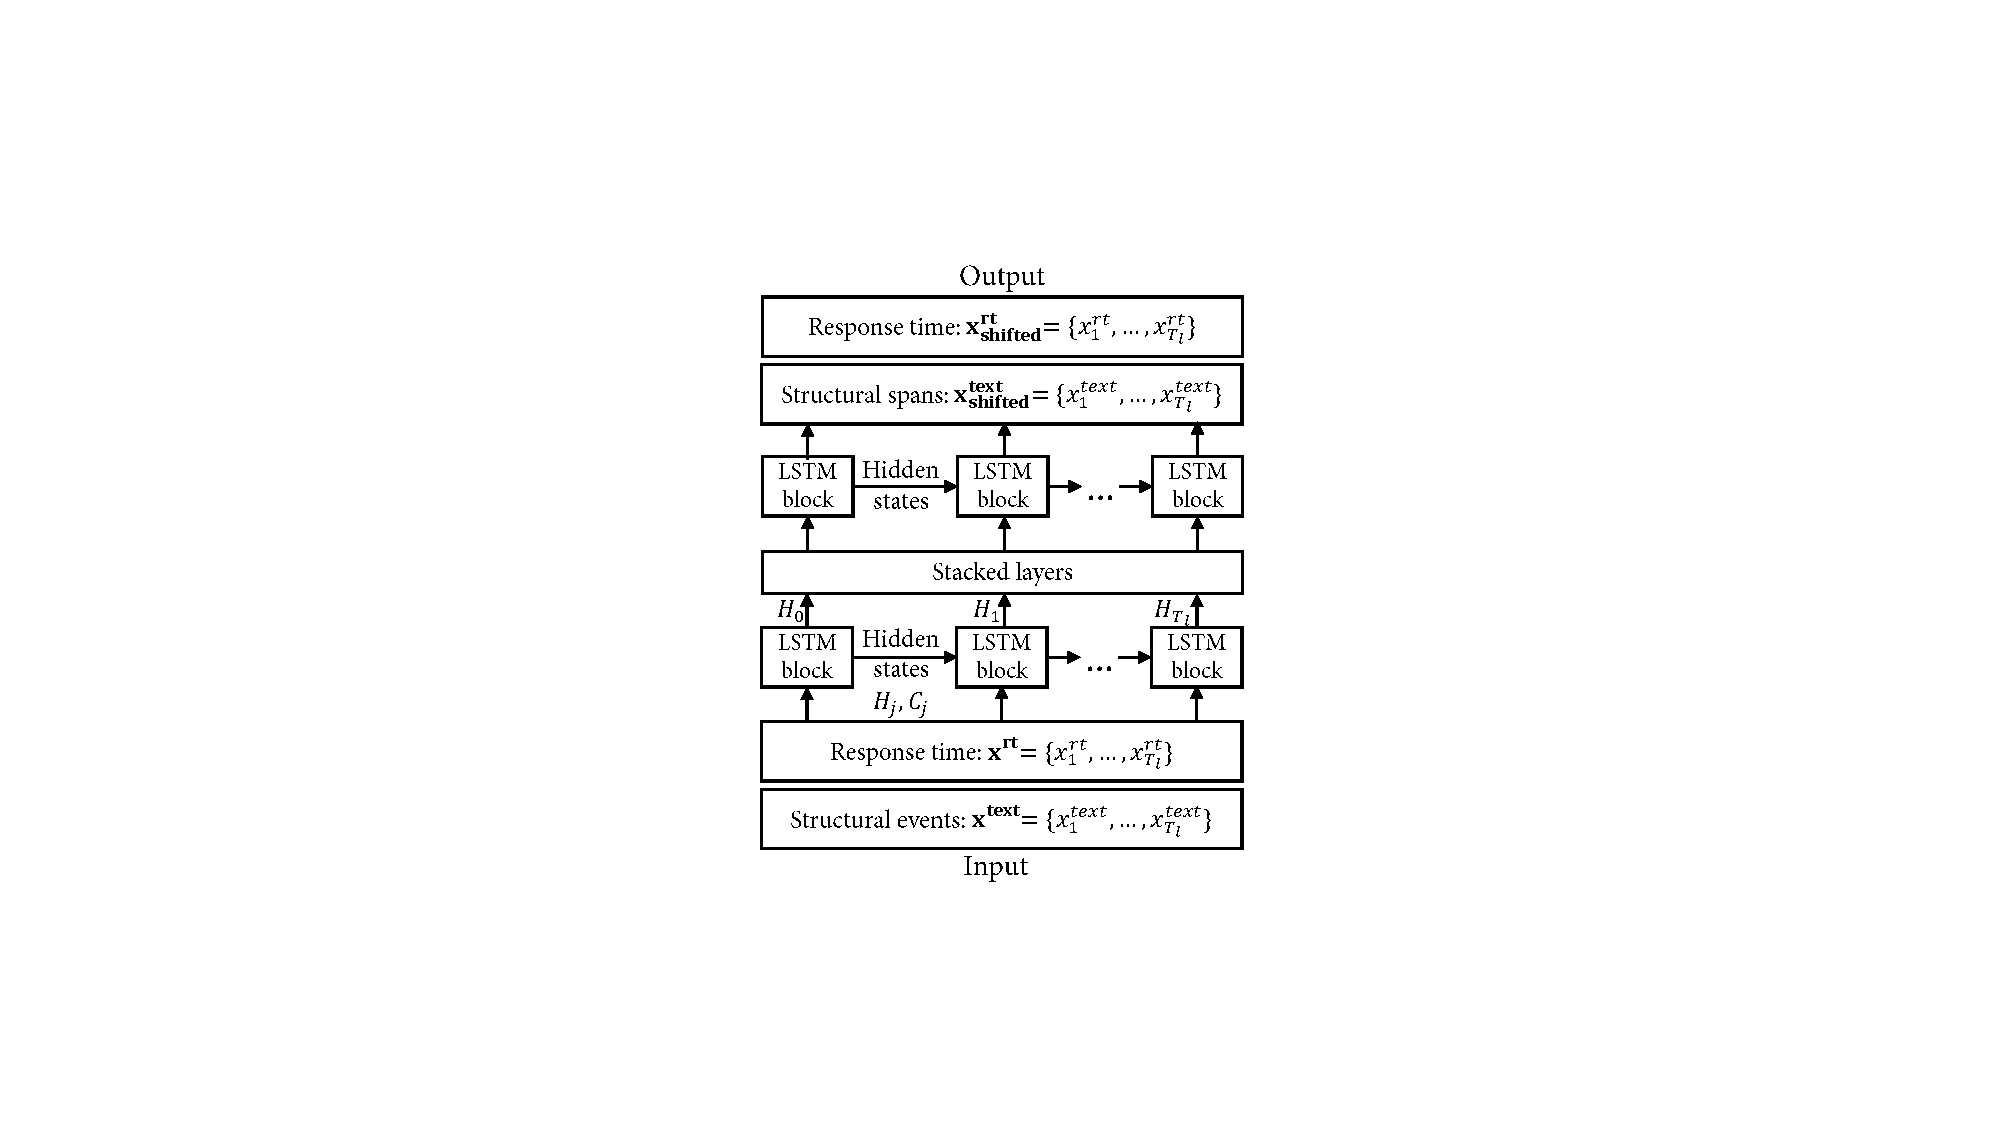
\includegraphics[width=0.6\textwidth]{gfx/chap6/singlemodality.pdf}}
\caption{Single-modality LSTM network architecture}
\label{lstmstructural}
\end{figure}

\subsection{Single-modality LSTM network} \label{singlemodal}

We denote the set of all unique labels in the data as $L=\{l_0, l_1, \dots, l_{N_l}\}$. Furthermore, $x_{i}^{text}$ denotes the one-hot encoding value of the label $l_j \in L$ positioned at index $i$ in the trace $\mathbf{x_i}$ for $i \in \{0, 1, \dots, N\}$. The value of $x_{i}^{text}$ depends on the trace structure prior to $x_{i}^{text}$, as the events in a trace originate from the execution of services upon a user request, where the events have a parent-child causal relationship~\cite{openzipkin}. We model the structural anomaly detection in traces as a sequence-to-sequence, multi-class classification problem, where each distinct label represents a class. Figure~\ref{lstmstructural} shows a single-modality architecture for both types of data $D_1$ (Structural Anomaly Detection, SAD) and $D_2$ (Response Time Anomaly Detection, RTAD). The detection of anomalies from a sequence of labels enables to capture the errors during the execution as well as to detect unexpected execution paths. 

The input to the model are the textual labels from a trace $\mathbf{x^{text}}$.
Each $x_i^{text}$ is fed as input in the corresponding timestep $time=i$. 
The output at $time=i$, for the current inputs $\{x_0^{text}, x_1^{text}, \dots, x_{i-1}^{text}\}$, is a probability distribution over the $N_l$ unique labels from $L$, representing the probability for the next label $x_i^{text}$ in the sequence. 
The detection phase uses this model to make a prediction and compares the predicted output against the observed label value. 
The LSTM network is trained to maximize the probability of each $x_{i}^{text},  (i\in \{1,2.. T_{l}\})$ to appear as a next label, i.e., minimizing the cross-entropy loss. 
Every LSTM block in Figure \ref{lstmstructural} at $time=i$ is composed of $h$ LSTM cells. 
It has a memory state that encodes all of the information from the previous timesteps together with the input fed at the same timestep.
LSTMs use different types of trainable gates~\cite{hochreiter1997long}, which together with the the input label at $time=i$ and the output from the previous block $H_{i-1}$ are used to decide:
\begin{itemize}
\item how much of the previous cell state $C_{i-1}$ should retain in its own state,
\item how to use the current input and the previous output $H_{i-1}$ to influence the state, and 
\item how to construct the output $H_{i}$.
\end{itemize}
In this manner, the possible extracted non-linear and temporal information is passed between adjacent LSTM blocks. 

The vertical stacking of layers as shown in Figure~\ref{lstmstructural} is a common practice in order to achieve better results by extracting highly-abstract features. We formulate each input-output pair from $D_1$ as $$\mathbf{x^{text}}=x_0^{text}, x_1^{text}, \dots, x_{T_l}^{text} \rightarrow \mathbf{x_{shifted}^{text}}=x_1^{text}, x_1^{text}, \dots, x_{T_l}^{text}$$ where the output is shifted by one event and concluded with the '\texttt{PAD}' label. These pairs are used to incrementally update the network's weights through categorical cross-entropy loss minimization via gradient descent.


\emph{Detection.} In order to evaluate, if a trace $\mathbf{X_{test}}$ represents an  anomaly and to discover, which events support the decision,is fed to the network's input. In each timestep, the network calculates a probability distribution:
$$P=\{l_0:p_0, l_1:p_1, \dots, l_{N_l}:p_{N_l}\}$$ 
describing the probability for each label from $L$ to appear as the next label value in the trace, given the previous values. The output layer of the network is composed of a soft-max function. It distributes the probability over the labels and ensures that $\sum_i^{N_l}{p_i} = 1$. 

Previously, we described that two or more events can be a result of multiple concurrent actions; therefore few of the possible labels can appear as the next label in the sequence. Comparison of the input label only to the most probable label can be a measure for the performance of the model in terms of the ability to capture the normal execution paths. For robustness, we compare the observed label to the $k$ predicted most probable labels: if the input label observed in the next timestep from the original sequence is not one of the top-$k$ labels with the maximum probability, then an anomaly is reported, i.e. the trained network has not observed a normal trace with the same or similar structure. Along with the information that the trace contains an anomalous execution path, we also provide the user with information which events contributed to the decision. This is important for further analysis tasks such as the root-cause analysis. 

\subsubsection{Response time anomaly detection (RTAD)}
The response time characterizing intra-service calls is decisive for the anomaly detection, as a sudden increase may indicate a problem with the involved service or with the underlying distributed system. The dependencies between the events in a trace affect the response times. Assume a service A calls other service B, collects the result, and proceeds with the execution (parent-child relationship). In this case, the second service is a service-child. Therefore, an increase or decrease in the child's response time will correspondingly lead to a change in the parent's response time. The ability to detect specific events that are anomalous in such perspective provides more insights and extends the range of the anomaly detection from the tracing data.

To extend the single-modality architecture to the multimodal LSTM, we first describe how to model the response time independently of the labels. Therefore, we reuse the neural network architecture presented in Figure~\ref{lstmstructural} and model the inter-event, response time dependencies in a trace using RTAD ($D_2$) data. The difference is that instead of the multi-class classification, the task is regression where the input and the output are real-valued numbers. In each timestep $time=i$, with $\mathbf{x^{text}}=x_0^{rt}, x_1^{rt}, \dots, x_{i-1}^{rt} $, the network predicts the response time $x_{i}^{rt}$ for the next event. In contrast to the structural anomaly detection, the weight updates are obtained through minimization of the mean squared loss via gradient descent. 

The detection is carried out by computing the squared error distance $error_i = (x_{i}^{rt}-\hat{x_{i}^{rt}})^2$, where $\hat{x_{i}^{rt}}$ is the predicted value at timestep $time=i$. Furthermore, similarly to the time series error threshold selection explained in \autoref{ch:metrics:sec:metano:subsec:threshold}, we separately model the error values for each label by fitting the Gaussian distribution. If the squared error between the prediction and the input at $time=i$ is out of the 95\% confidence interval obtained from the Gaussian, the event and the trace are flagged as anomalous.

\begin{figure}[htbp]
\centerline{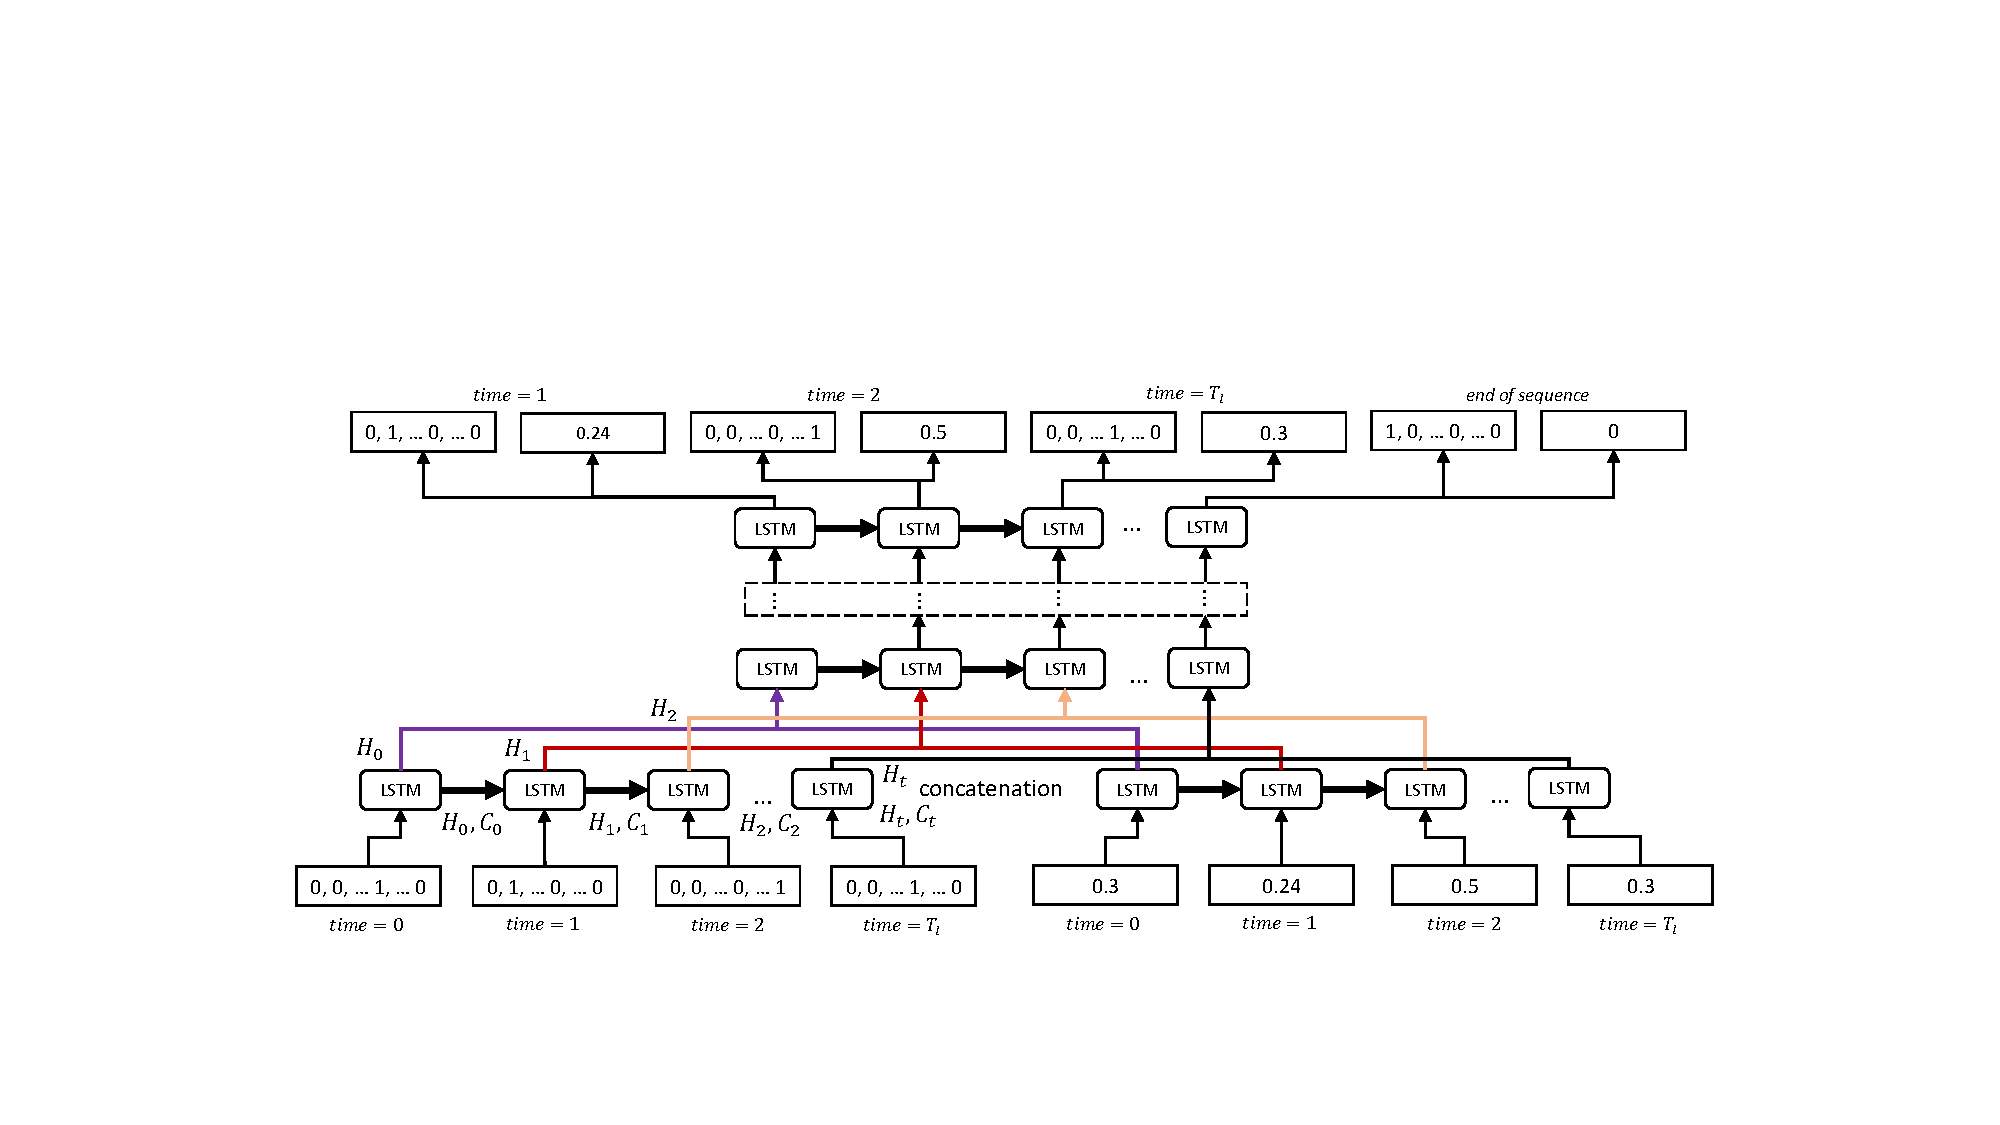
\includegraphics[width=1.0\textwidth]{gfx/chap5/multitasklstm.pdf}}
\caption{Multimodal LSTM neural network architecture for anomaly detection from complete tracing data}
\label{lstmmultitask}
\end{figure}

\subsection{Multimodal LSTM}\label{multimodal}
The response time together with the event's label completely characterizes a single event. The correlation between these two types of data motivates the need to use both modalities of the data in a single model aiming to extend the anomaly detection for tracing data and to achieve a better overall accuracy. 

The proposed multimodal LSTM architecture is assembled as a horizontal concatenation of both single-modality architectures, as shown in Figure \ref{lstmmultitask}. The model contains two data modalities as inputs: $D_1$ and $D_2$. From the bottom-up perspective of the architecture, we have layer with LSTM blocks for each input. We perform the concatenation in the second hidden layer. The concatenation can be carried out in any hidden layer chosen by cross-validation. The merging of the two modalities is done in the following way: LSTM outputs from the first layer in $time=i$ are joined and forwarded into the same timestep in the next LSTM layer. In Figure \ref{lstmmultitask}, the color-coding scheme represents the concatenated pairs. 

Starting from the concatenated layer, the information is jointly encoded and flows between modalities. From this joint representation, the many-to-many neural network learns the mapping to the outputs. The input-output pairs can be formalized as:

$$input=[\{\mathbf{x^{text}}=x_0^{text}, x_1^{text}, \dots, x_{T_l}^{text}\}, \{\mathbf{x^{text}}=x_0^{rt}, x_1^{rt}, \dots, x_{T_l}^{rt} \}] $$
$$\rightarrow output=[\{\mathbf{x^{text}}=x_1^{text}, x_2^{text}, \dots, x_{T_l}^{text}, \mathrm{PAD}\}, \{\mathbf{x^{rt}}=x_1^{rt}, x_2^{rt}, \dots, x_{T_l}^{rt}, \mathrm{PAD}\}]$$

In the training phase, we use different cost functions for the modalities. The input-output pairs are used to learn the weight updates through minimization of a joint loss which is the sum of the mean squared error for the response time and the categorical cross-entropy for the labels. 

\emph{Detection.} The detection in the multimodal setting is performed by comparing the output element-wise with the input for both modalities using the strategy developed in the single-modality architectures. An advantage is that with a single model we can detect anomalies in both modalities, overcoming the limitations of not having a single-modality response time anomaly detection. For example, when there is an increased response time in one of the events, and the computed error between the prediction and the input is out of the confidence interval, the method reports an anomaly. Similarly to the SAD, if the observed input labels of the sequence are not in the top-$k$ element-wise predictions, an anomaly is reported. Considering the both modalities, the anomaly type can be either: response time anomaly, structural anomaly, or anomaly in both modalities. It is worth noting that the anomaly in the response time can be independent of the structure and vice versa.

\subsection{Detection of Dependent and Concurrent Events}
The output of structured anomaly detection model encodes the underlying execution path. Every label predicted as the label for the next event in the trace describes a probability distribution of all possible labels. The events have a parent-child relationship, which can be extracted from the recorded data. However, the challenge of recognition of concurrent and dependent events in the execution path is not solved yet and has to be addressed.

Considering that the neural network learns the underlying execution paths (i.e. the causal relationship between the events), we can reconstruct them using the predicted probability distribution over the labels, similar to the approach presented in Figure~\ref{workflow}. Assume we aim to predict the event in the trace next to the vertical, dashed line. The input at timestep $time=3$ is $\{x_1^{text}, x_3^{text}, x_8^{text}, x_{12}^{text}\}$. Let the top-2 probabilities for the next label in the sequence be $P(\hat{x_6^{text}})=0.55, P(\hat{x_{11}^{text}})=0.45\}$, while for the rest of them, the probability is zero. In order to determine if these two events are produced as a result from concurrently invoked services we analyze two different inputs: $\{x_1^{text}, x_3^{text}, x_8^{text}, x_{12}^{text}, x_{6}^{text}\}$ and $\{x_1^{text}, x_3^{text}, x_8^{text}, x_{12}^{text}, x_{11}^{text}\}$. If for both sequences the probability for the next label is $P(x_{2}^{text})=1.0$, the events (services) are concurrent as both of them lead to the same event.   

We also discuss a mechanism to detect dependent events. In this case, if the probability to observe $x_{i}^{text}$ as a label for the next event in the sequence is one, then $x_{i}^{text}$ and $x_{i-1}^{text}$ are dependent. 

\begin{figure}[htbp]
\centerline{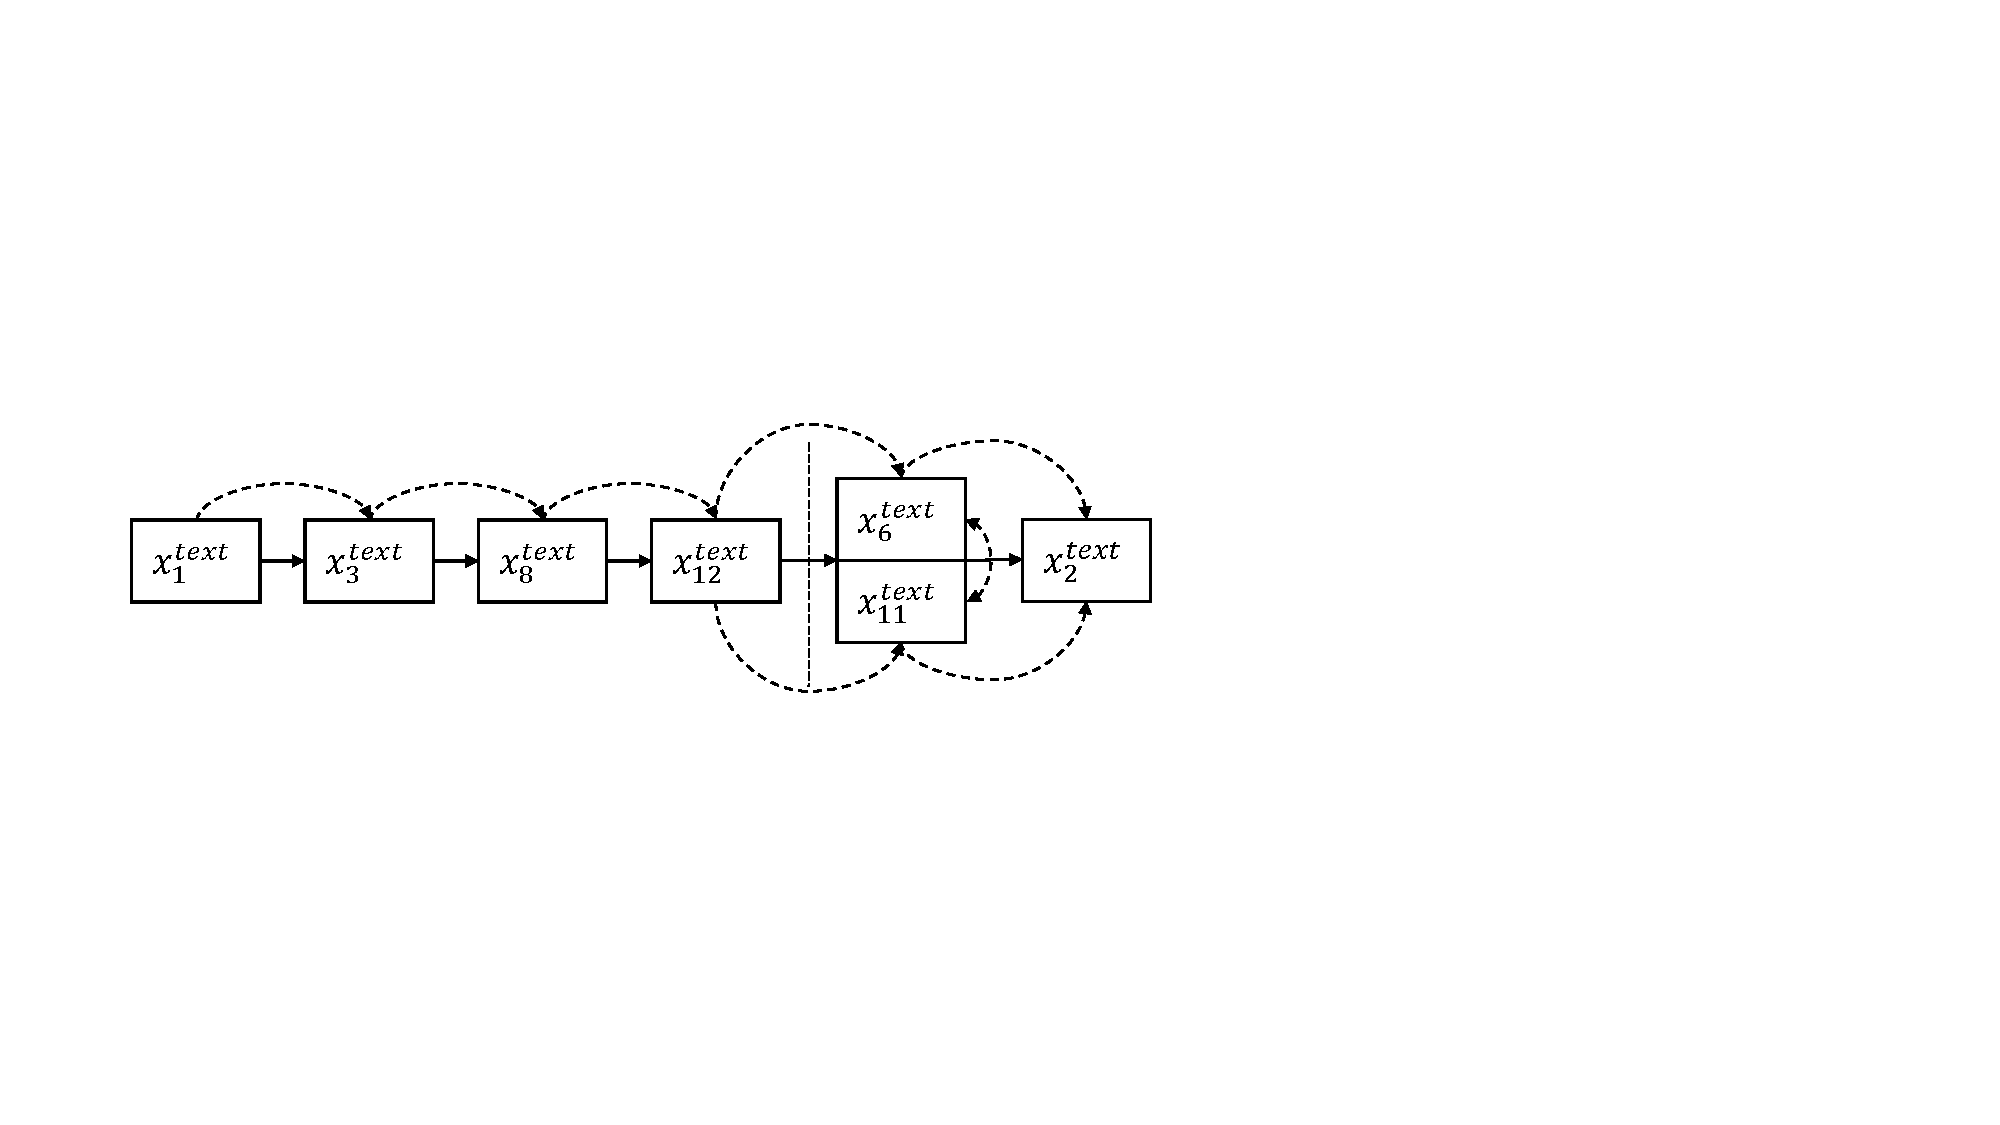
\includegraphics[width=1.0\textwidth]{gfx/chap6/dependentconcurrent.pdf}}
\caption{Trace execution path with concurrent events.}
\label{workflow}
\end{figure}

\section{Evaluation}\label{evaluation}
The methods were implemented in Python using Keras~\cite{chollet2015keras}. The experiments on the collected dataset were carried out on regular personal computer using GPU-NVIDIA GTX 1060 6GB, 1TB HDD, 256 SSD, and Intel(R) Core(TM) i7-7700HQ CPU at 2.80 GHz.

\subsection{Experimental Setup}
In this section, the dataset utilized for trace anomaly detection will be described. Next, we present the types of anomalies that are injected into the system, and the baseline methods.

\subsubsection{Dataset 1: large production cloud data}
The data was collected from a production cloud platform which runs Openstack \cite{ShrivastwaOpenstack} with Zipkin \cite{openzipkin} as a tracing technology. With more than 1000 micro services, the underlying system enables an exhaustive and realistic evaluation of our approach. The collected traces are recorded over a period of 50 days, yielding over 4.5 million events distributed in more than one million traces with different lengths. 

The JSON objects representing the events, are parsed and the two different data modalities $D_1$ and $D_2$ are compiled. To avoid outliers, we select labels that appear more than 1000 times in the data, making a total of 105 unique labels. The distribution of the trace lengths in our dataset is imbalanced; more than 90\% of the traces have lengths smaller than 10 events. This is compensated by selecting only 1000 samples of each trace length, where the trace lengths with less samples are completely included into the dataset. In this regard, our approach requires approximately less than 1\% of all the recorded data, which makes it efficient and fast for training. 

\begin{figure}[htbp]
\centerline{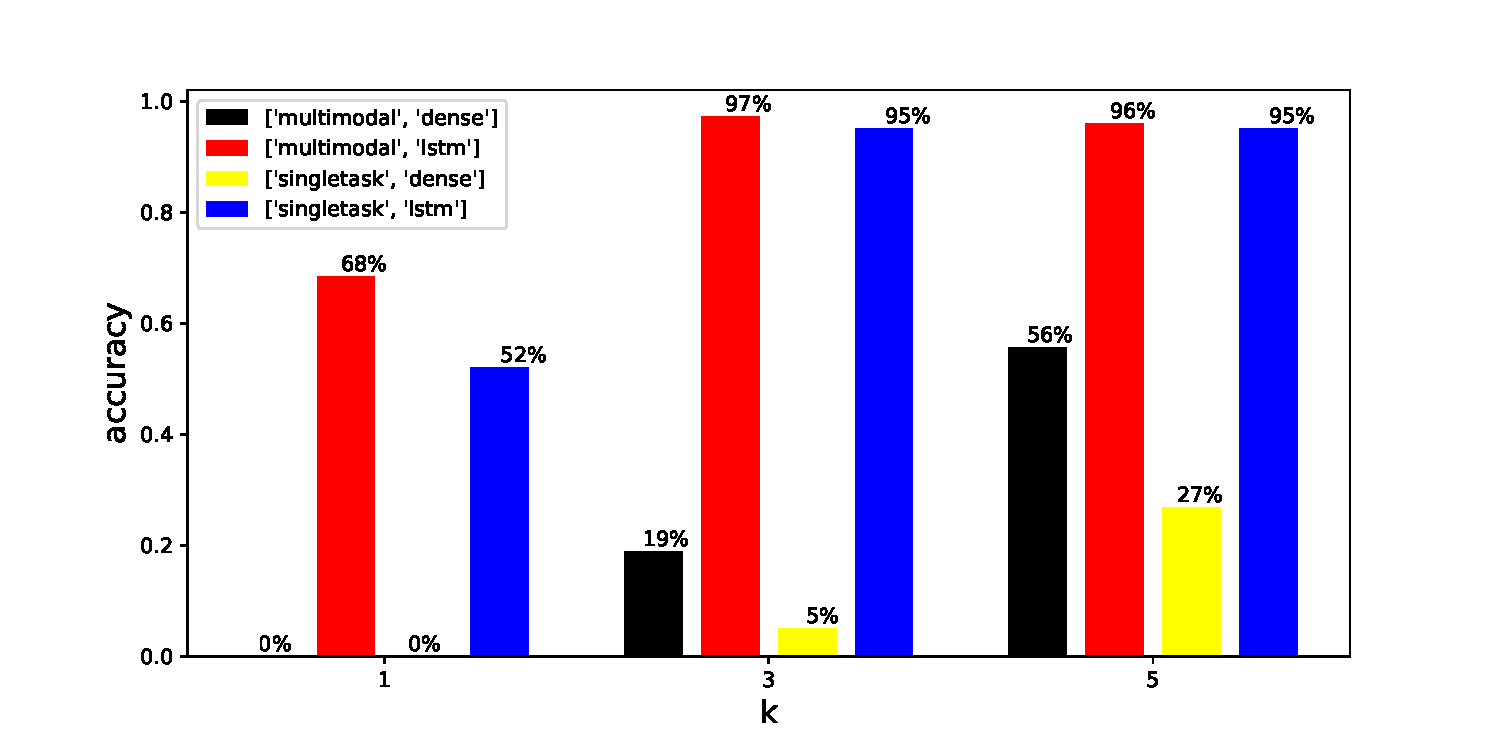
\includegraphics[width=1.0\textwidth]{gfx/chap5/groupbyk.pdf}}
\caption{Comparison of the overall accuracies of the models evaluated for three values of $k \in \{1, 3, 5\}$.}
\label{k}
\end{figure}

\begin{figure}[htbp]
\centerline{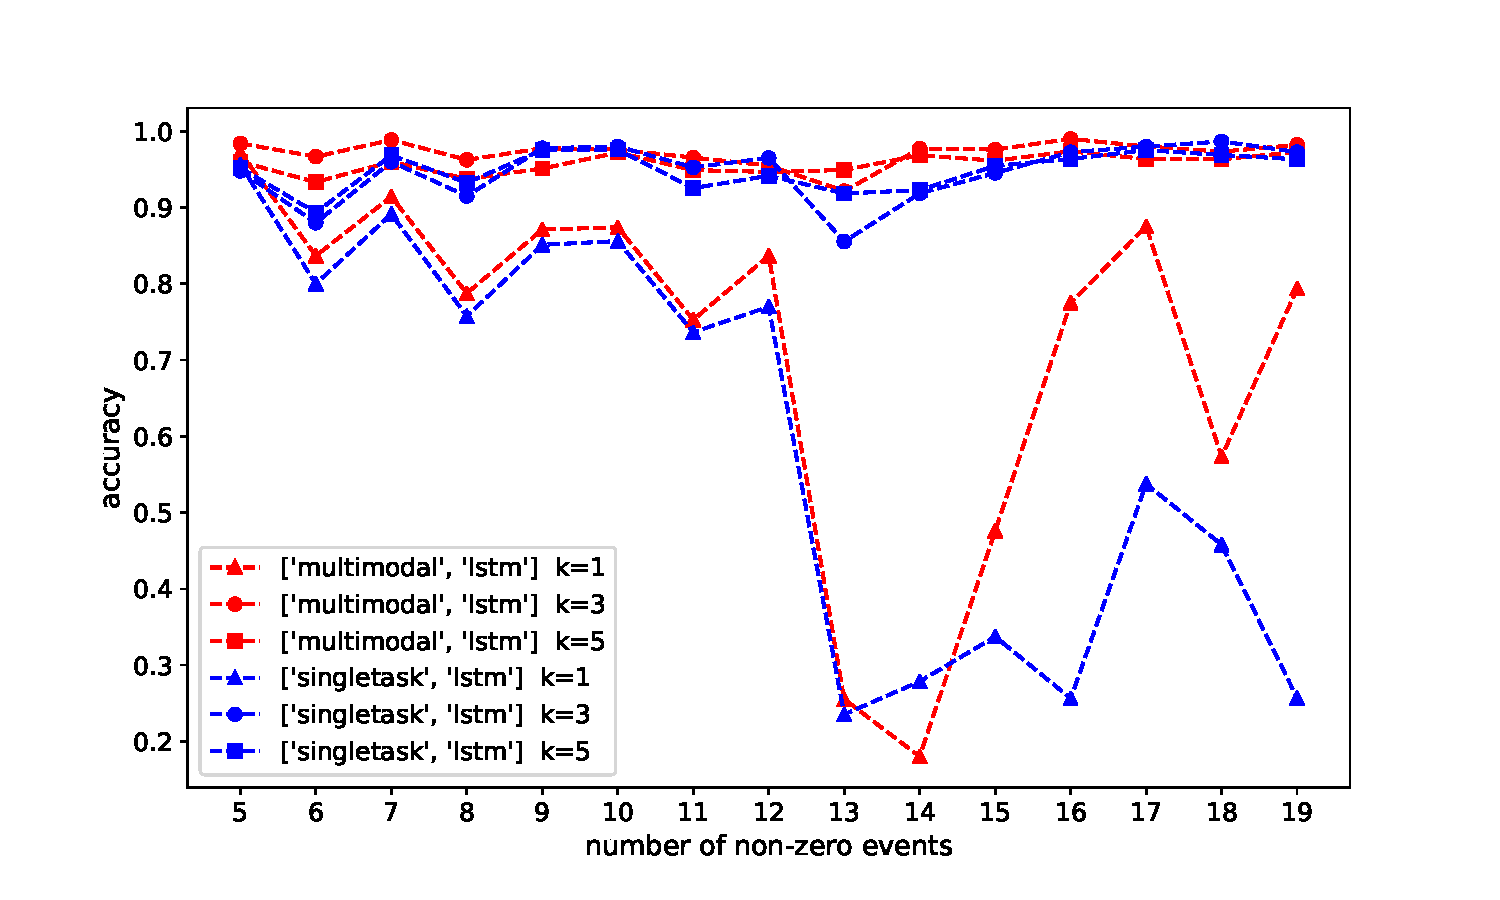
\includegraphics[width=1.0\textwidth]{gfx/chap5/groupbykn.pdf}}
\caption{Comparison of the accuracies of two best models, evaluated for each trace length \(4-20\)
and $k \in \{1, 3, 5\}$.}
\label{kn}
\end{figure}

\begin{figure}[htbp]
\centerline{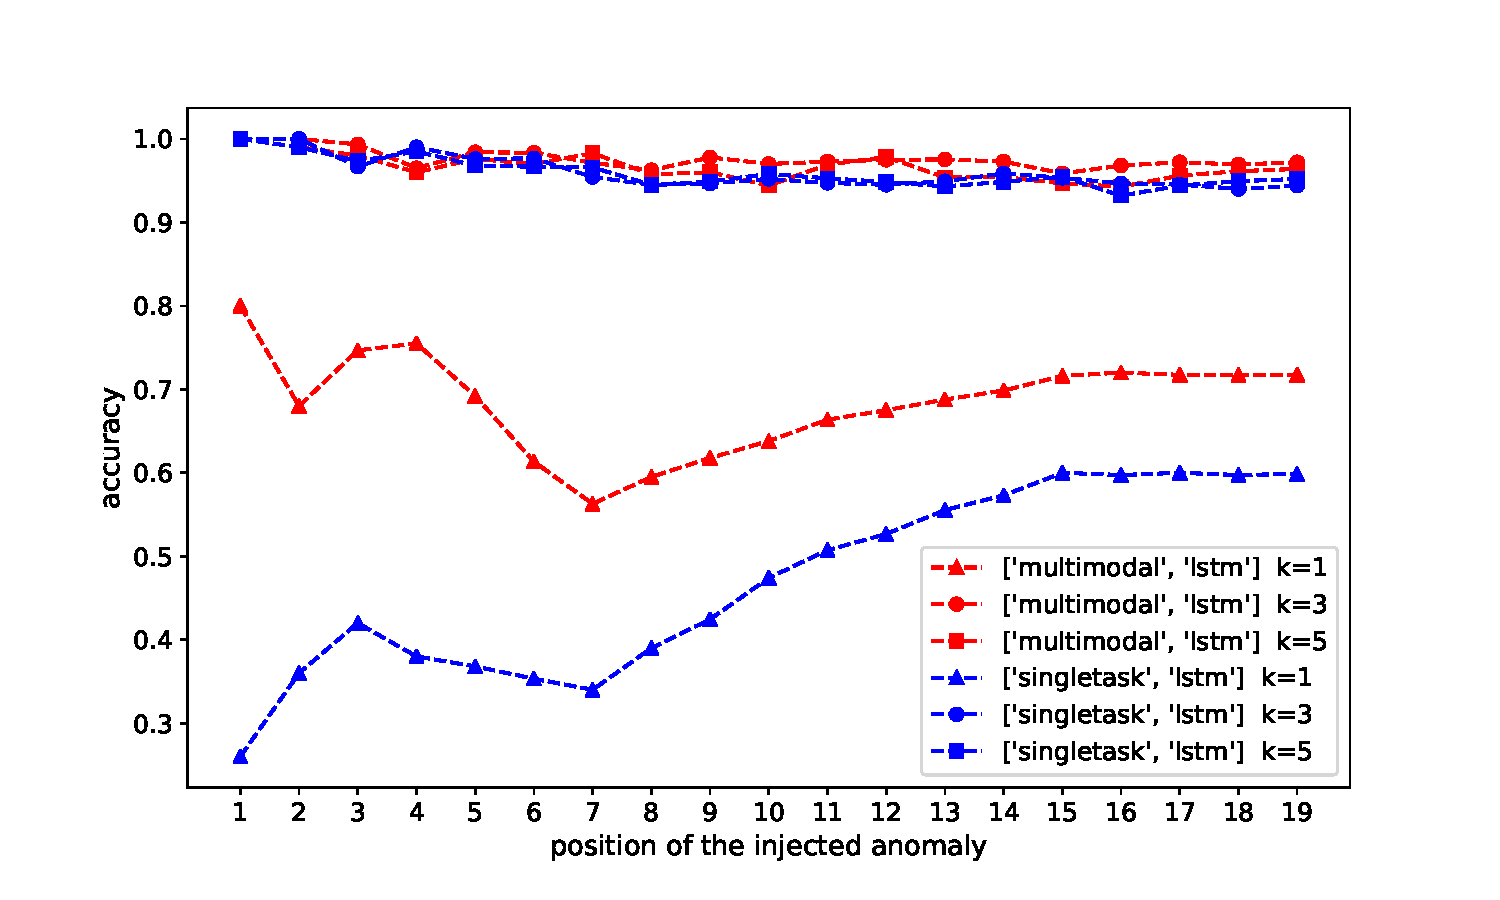
\includegraphics[width=1.0\textwidth]{gfx/chap5/groupbykidx.pdf}}
\caption{Comparison of the accuracy of the two best models, evaluated for different positions \(0, 20\) of the injected anomaly and $k \in \{1, 3, 5\}$.}
\label{kidx}
\end{figure}

\emph{Anomaly Injections and Measurement of Accuracy for SAD.} The accuracy evaluation for detected anomalies is carried out by artificially injecting anomalies in the data. For SAD, we performed anomaly injections as follows: given a trace $T_{test} = \{e_0, e_1, \dots, e_{T_l}\}$, with $N_z$ non-zero elements and top-$k$ predictions for each position $i$ in the trace, we select a label, which is not in the top-$k$ predictions, and inject it at the position of the normal observed label. We then run the prediction with the model and determine a decision anomaly/normal by comparing the non-corrupted sample with the prediction. In case of output \textit{true} and the label in the corrupted event position is not in the top-k predictions, the injected anomaly is successfully detected.

\emph{Anomaly Injections and Measurement of Accuracy for RTAD.} We perform the anomaly injections by selecting the event response time $rt_i$ at a position $i$ of the trace. The anomaly is injected by increasing the response time of the event by a random value $r \in (2*rt_i, 5*rt_i)$. Once the anomaly is injected, we compute the mean squared error between the input and the predicted output. If the error is not in the 95\% confidence interval computed from the Gaussian fitted on the training set, then the anomaly is detected successfully. 
The accuracy is computed as the ratio of the number of successfully detected anomalies and the number of injected anomalies.

In practice, the anomaly may not appear only in a single event. We assume that a trace is anomalous if at least one event inside deviates from the normal behavior, making our approach applicable when the anomaly is spread across multiple events. 

\emph{Baselines.} We have two baseline models for comparison, single- and multimodal deep learning architectures composed of simple feed-forward neural networks. The architecture for the single-modality network is {input, dense(50), dense(20), output}, while for the multimodal is {[$D_1$-input, $D_2$-input], dense(50) for $D_1$, dense(50) for $D_2$, concatenation, dense(20) for each, output for each}. The decision for anomaly is done in the same way as previously described.

\subsection{Results and discussion}


\begin{figure}[htbp]
\centerline{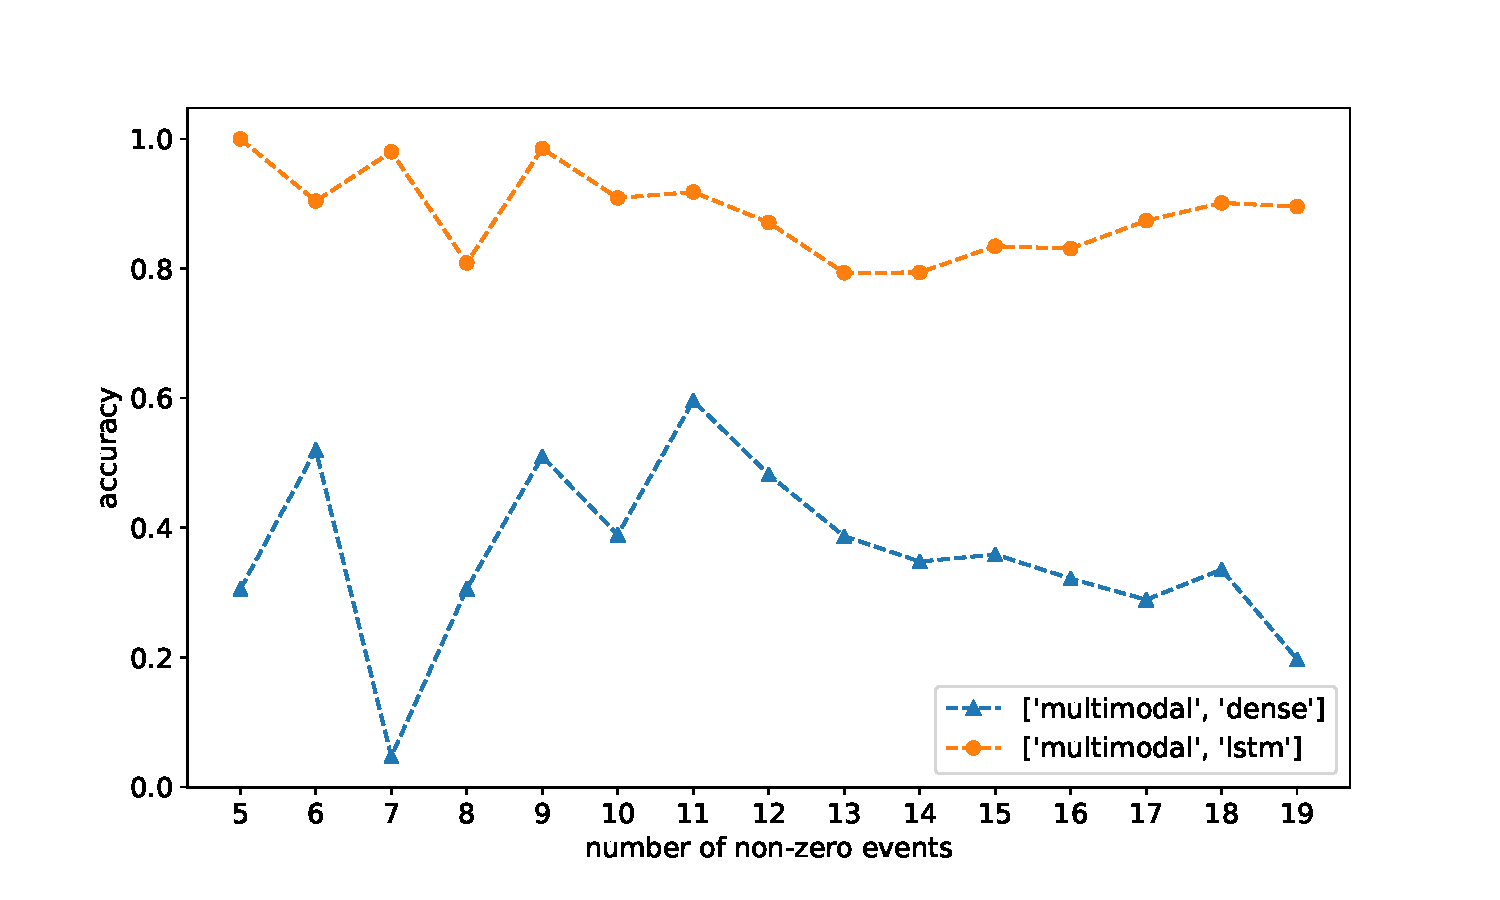
\includegraphics[width=1.0\textwidth]{gfx/chap5/rtnonzero.pdf}}
\caption{Response time anomaly detection accuracy comparison of the multimodal LSTM and the baseline deep learning architecture evaluate for different trace lengths.}
\label{rtnonzero}
\end{figure}


As shown in Figure \ref{k}, the best results in terms of accuracy for the task of structural anomaly detection are achieved using the multimodal LSTM predictions. The bar plot shows the accuracy of all models when different values of $k$ are used. We observe that that the single-modality LSTM achieves a comparable accuracy, while the other two single- and multimodal dense architectures have low accuracies. The dense models can not take into account the temporal information. Compared to that of the single-modality LSTM architecture, the multimodal LSTM achieves a better accuracy owing to the additional response time information. The results for $k=3$ and $k=5$ are comparable, while the results for $k=1$ show that the multimodal approach outperforms the single-modality by a large margin of 16\%. Because of the low percentages obtained from the traditional models, we do not compare them below. 

We evaluated the accuracy when the anomaly is injected in traces with different sizes, as shown in Figure \ref{kn}, while ignoring the position of injection of the anomaly. Both proposed architectures achieve high accuracies for $k \in \{3,5\}$. The multimodal slightly outperforms the single-modality approach in 9 out of 15 trace lengths for both $k$. Significantly better results are achieved for $k=1$ for almost all of the trace lengths. The plot demonstrates that both approaches are stable, without performance reduction when the trace length is increased.

Further, for SAD, we compared the two best models when the anomaly is injected in different positions in the trace for $k \in {1,3,5}$, while ignoring the trace length. Similarly, Figure \ref{kidx} shows a significantly better performance of the multimodal approach for $k=1$. Furthermore, the accuracy is also stable at all of the different positions of the trace. This implies that the model successfully detects injected anomalies for different events in different positions of the trace.

\begin{figure}[htbp]
\centerline{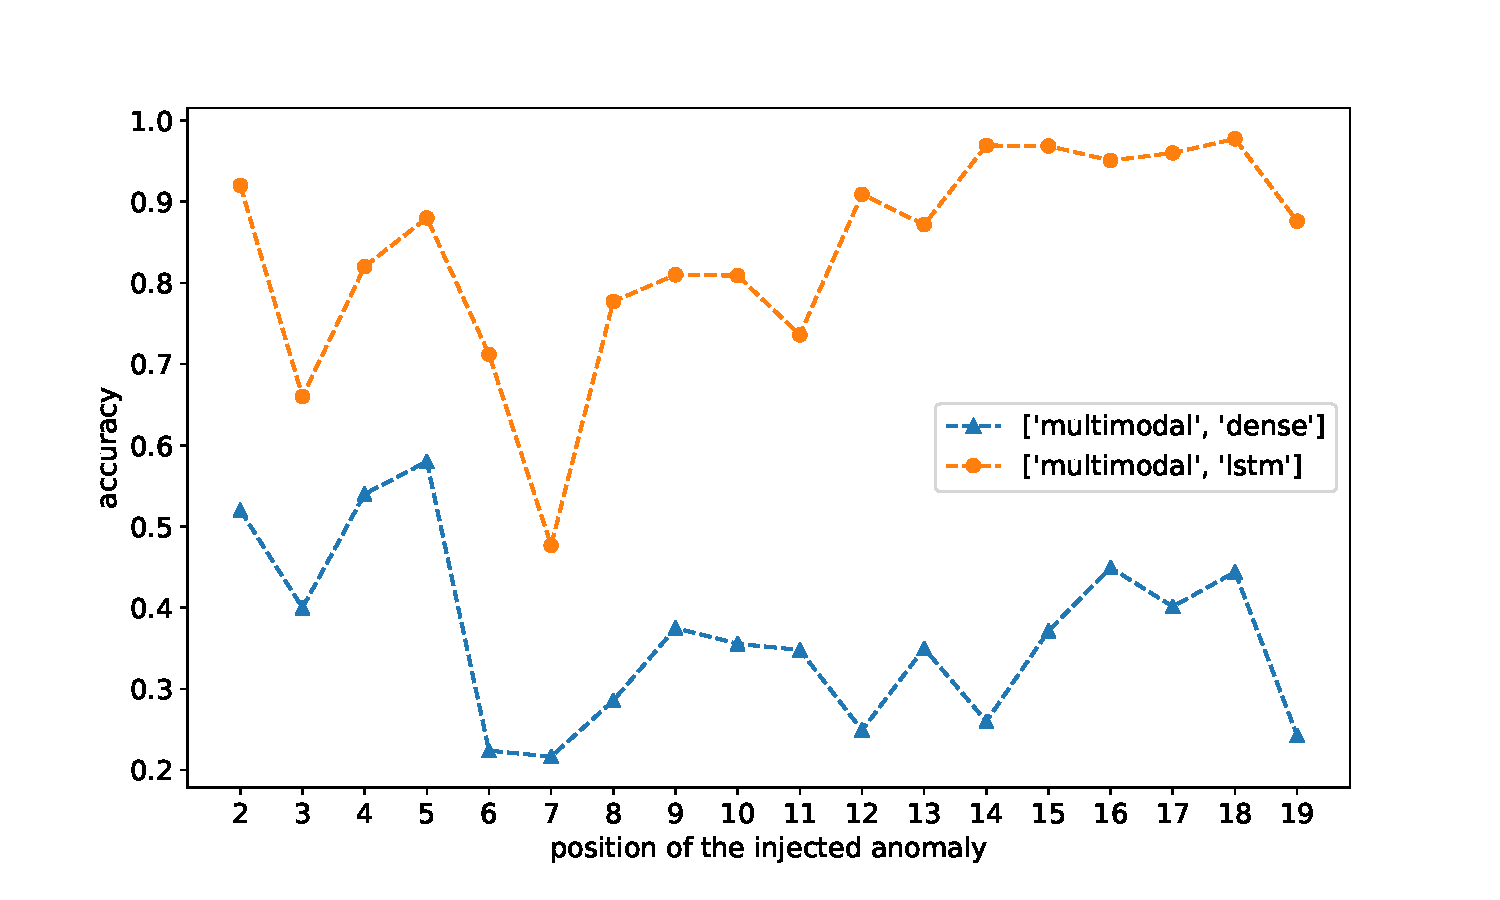
\includegraphics[width=1.0\textwidth]{gfx/chap5/rtidx.pdf}}
\caption{Response time anomaly detection comparison between the multimodal LSTM and the baseline deep learning architecture, evaluated for different positions of the injected anomaly.}
\label{rtidx}
\end{figure}


\emph{RTAD.} The single-task models for sequential response time modelling have quite low performances than those of both multimodal models, and thus we discuss only those results. Figures \ref{rtidx} and \ref{rtnonzero} show comparisons of the two multimodal approaches for different positions of the injected anomaly and different trace lengths.  In both figures, the multimodal approach achieves a higher accuracy for response time anomaly detection. Figure \ref{rtnonzero} shows that the accuracy slightly decreases when the trace length is larger. In Figure \ref{rtidx}, the reason why the accuracy drops at position 7 is because of the small signal-to-noise ratio and the existence of outliers. In our approaches, we have not applied any preprocessing or outlier removal techniques, but we assumed that the recorded data represent the normal behavior. The use of preprocessing techniques for the response time may eventually help improve the accuracy for the response time in critical positions.

The models are consistent and have high accuracy even when the length of the trace increases. This is because of the LSTMs which are able to learn long-term dependencies in sequential tasks.

\emph{Performance.} The time needed to train the multimodal LSTM on the 1\% representative sub-sample of over one million traces was approximately 30 min. The model is applicable for real-time anomaly detection with a prediction time per trace below 50 ms.

\section{Related Work} \label{related_work}
Prior of the introduction of deep learning methods for trace anomaly detection, mostly rule based methods are found in the literature. 
Tracing technologies for distributed services record information about all the individual components participating on an e.g., user request (initiator) within the system.
Two classes of solutions have been proposed to aggregate these information so that one can associate all record entries with a given initiator, black-box and annotation-based monitoring schemes \cite{36356}. Black-box schemes \cite{reynolds2006wap5, bahl2007towards, aguilera2003performance} assume there are no additional information other than the message record described above, and use statistical regression techniques to infer that association. Annotation-based schemes \cite{gschwind2002webmon, Fonseca:2007:XPN:1973430.1973450, aguilera2003performance, barham2003magpie} rely on applications or middleware to explicitly tag every record with a global identifier that links these message records back to the originated request.

While the anomaly detection on other categories of data like log and metric are part of previous research \cite{8456348, 8457902,du2017deeplog, bezerra2013algorithms, brown2018recurrent, mining-invariants-from-console-logs-for-system-problem-detection, 6008688}, the  related work on anomaly detection in trace data is still limited.

In ~\cite{RepTrace}, a method for anomaly detection in distributed traces is presented. The complete path of processing a specific service/job request is represented by a Request Execution Path (REP). The main aim is to build a pair of finite-state automata (FSM) for each type of workload represented by the REP. One of the FSM’s represents the maximal common subpattern of spans from a type of workload, while the other FSM represents all the possible combinations as appearing in the training set. Since the workload is known in advance during the anomaly detection phase just the respective pair of FSM for anomaly detection is invoked. The anomaly is detected as the absence of state transition from a given state in the full FSM or after no change in the state space of the core FSM during a period of 5 seconds. 
This approach is expected to have issues for long traces. The FSM for the long traces can be too complex and hurt the performance of the method. Although they address this problem with the inclusion of pruning which acts like discarding information from the data. One workload can have a different order of representation of the spans if originates from a production data due to various reasons e.g caching. Since the FSM defines determinism between the state transitions, the different order in which the spans arrive can have a strong implication on the invocation order between the states in the FSM. Thus, the determinism is a strong assumption in real-world scenarios. 

In~\cite{fu2009execution}, the authors present an approach for anomaly detection in distributed systems build on the FSM. It builds the FSM on each system module. As input to this method are given logs originating from a component with a componentID, meaning that they can be treated as a form of a trace. The logs are first parsed and represent as integer templates. Then are used to build the FSM. During the anomaly detection phase, if the input sequence presented to the FSM can be generated by it, then the input sequence is considered normal otherwise it is an anomaly. 
This method requires building an FSM for each system component. This can be an expensive procedure. Furthermore, it does not address the problem of long traces and cannot take into consideration the interaction between the different components in the system since the FSM is built on system component (module) level. Thus, it does not preserve the information about the interaction between the components. Our solution is request centric since it utilizes distributed traces. This allows modelling the interaction between the components (services) as compared to the previously mentioned approach.

In~\cite{eskin2002geometric} an unsupervised anomaly detection method from system tracing data is presented. To preserve the sequence within the system trace data a specialized kernel function tailored for sequential data is adopted. This kernel function allows for implicit mapping of the original sequential traces into a higher dimensional space while preserving the sequential properties. The decision of the anomaly is done with calculation of the distances of the new point in the higher dimensional space to the “dense”-normal and “sparse”-abnormal clusters learned during the training phase of the method. Based on the closer cluster, a decision for the trace is made. 
A drawback of this approach is the need to specify the kernel function in advance. The assumption of the kernel function implies learning of fixed implicit mapping. This relates to absence of flexibility since the kernel function should always be changed to best adapt the input traces. In comparison our method allows for learning the mappings to higher dimensional space, as opposed to pre-specifying the possible mapping. This makes the method more flexible to the input data as opposed to this art.  

In contrast to the above anomaly detection systems, we presented a single model that utilizes the multimodal nature of the trace data. Referring to our work, TraceAnomaly, Our core idea
is to use machine learning to automatically learn the overall normal patterns of traces during periodic offline training. In online anomaly detection, a new trace with a small anomaly score (computed based on the learned normal pattern) is considered anomalous. They design a deep Bayesian network with posterior flow where they show that they can accurately and robustly detect trace anomalies in a unified fashion on traces from a bank software. They evaluated our work~\cite{nedelkoski2019anomalymultimodal}, on the proprietary dataset, showing near state-of-the-art results in structural trace anomaly detection.

\section{Chapter Summary} \label{conclusion}
This chapter addressed an important and growing challenge from the field of AIOps: the anomaly detection in large-scale cloud infrastructures using tracing data that contains detailed information about inter-service calls.

We addressed the problem using sequential deep networks for structural anomaly detection and  presented approaches to recognize dependent or concurrently invoked services. We further extended the approach by an architecture for multimodal anomaly detection. This approach enables to detect structural and response time anomalies by simultaneously considering the trace structure and the latency of the services.   

Our evaluation with data from a real-world production cloud showed that our multimodal LSTM  approach achieved over 90\% accuracy in multiple experiments, outperforming the single-modality and the baseline dense neural networks, although the single-modality LSTM yielded comparable results in structural anomaly detection.

Our approach paves the way for development of new techniques that simultaneously consider application logs, resource metrics, or other observability data to create a joint representation of states to enable the anomaly detection in large-scale complex microservice systems. These achievements are fundamental for the development of fully automated AIOps solutions for the automated anomaly detection, root-cause analysis, and remediation.